%!TeX encoding = UTF-8 Unicode
\documentclass[notheorems, aspectratio=54]{beamer}
% aspectratio: 1610, 149, 54, 43(default), 32
\usepackage[utf8]{inputenc}
\usepackage[english, vietnamese]{babel}
\usepackage{latexsym}
\usepackage{amsmath,amssymb}
\usepackage{mathtools}
\usepackage{color,xcolor}
\usepackage{graphicx}
\usepackage{algorithm}
\usepackage{amsthm}
\usepackage{lmodern} % 解决 font warning
% \usepackage[UTF8]{ctex}
\usepackage{animate} % insert gif

\usepackage{lipsum} % To generate test text 
\usepackage{ulem} % 下划线,波浪线

\usepackage{listings} % display code on slides; don't forget [fragile] option after \begin{frame}

% ----------------------------------------------
% tikx
\usepackage{framed}
\usepackage{tikz}
\usepackage{pgf}
\usetikzlibrary{calc,trees,positioning,arrows,chains,shapes.geometric,%
	decorations.pathreplacing,decorations.pathmorphing,shapes,%
	matrix,shapes.symbols}
\pgfmathsetseed{1} % To have predictable results
% Define a background layer, in which the parchment shape is drawn
\pgfdeclarelayer{background}
\pgfsetlayers{background,main}

% define styles for the normal border and the torn border
\tikzset{
	normal border/.style={orange!30!black!10, decorate, 
		decoration={random steps, segment length=2.5cm, amplitude=.7mm}},
	torn border/.style={orange!30!black!5, decorate, 
		decoration={random steps, segment length=.5cm, amplitude=1.7mm}}}

% Macro to draw the shape behind the text, when it fits completly in the
% page
\def\parchmentframe#1{
	\tikz{
		\node[inner sep=2em] (A) {#1};  % Draw the text of the node
		\begin{pgfonlayer}{background}  % Draw the shape behind
			\fill[normal border] 
			(A.south east) -- (A.south west) -- 
			(A.north west) -- (A.north east) -- cycle;
\end{pgfonlayer}}}

% Macro to draw the shape, when the text will continue in next page
\def\parchmentframetop#1{
	\tikz{
		\node[inner sep=2em] (A) {#1};    % Draw the text of the node
		\begin{pgfonlayer}{background}    
			\fill[normal border]              % Draw the ``complete shape'' behind
			(A.south east) -- (A.south west) -- 
			(A.north west) -- (A.north east) -- cycle;
			\fill[torn border]                % Add the torn lower border
			($(A.south east)-(0,.2)$) -- ($(A.south west)-(0,.2)$) -- 
			($(A.south west)+(0,.2)$) -- ($(A.south east)+(0,.2)$) -- cycle;
\end{pgfonlayer}}}

% Macro to draw the shape, when the text continues from previous page
\def\parchmentframebottom#1{
	\tikz{
		\node[inner sep=2em] (A) {#1};   % Draw the text of the node
		\begin{pgfonlayer}{background}   
			\fill[normal border]             % Draw the ``complete shape'' behind
			(A.south east) -- (A.south west) -- 
			(A.north west) -- (A.north east) -- cycle;
			\fill[torn border]               % Add the torn upper border
			($(A.north east)-(0,.2)$) -- ($(A.north west)-(0,.2)$) -- 
			($(A.north west)+(0,.2)$) -- ($(A.north east)+(0,.2)$) -- cycle;
\end{pgfonlayer}}}

% Macro to draw the shape, when both the text continues from previous page
% and it will continue in next page
\def\parchmentframemiddle#1{
	\tikz{
		\node[inner sep=2em] (A) {#1};   % Draw the text of the node
		\begin{pgfonlayer}{background}   
			\fill[normal border]             % Draw the ``complete shape'' behind
			(A.south east) -- (A.south west) -- 
			(A.north west) -- (A.north east) -- cycle;
			\fill[torn border]               % Add the torn lower border
			($(A.south east)-(0,.2)$) -- ($(A.south west)-(0,.2)$) -- 
			($(A.south west)+(0,.2)$) -- ($(A.south east)+(0,.2)$) -- cycle;
			\fill[torn border]               % Add the torn upper border
			($(A.north east)-(0,.2)$) -- ($(A.north west)-(0,.2)$) -- 
			($(A.north west)+(0,.2)$) -- ($(A.north east)+(0,.2)$) -- cycle;
\end{pgfonlayer}}}

% Define the environment which puts the frame
% In this case, the environment also accepts an argument with an optional
% title (which defaults to ``Example'', which is typeset in a box overlaid
% on the top border
\newenvironment{parchment}[1][Example]{%
	\def\FrameCommand{\parchmentframe}%
	\def\FirstFrameCommand{\parchmentframetop}%
	\def\LastFrameCommand{\parchmentframebottom}%
	\def\MidFrameCommand{\parchmentframemiddle}%
	\vskip\baselineskip
	\MakeFramed {\FrameRestore}
	\noindent\tikz\node[inner sep=1ex, draw=black!20,fill=white, 
	anchor=west, overlay] at (0em, 2em) {\sffamily#1};\par}%
{\endMakeFramed}

% ----------------------------------------------

\mode<presentation>{
	\usetheme{CambridgeUS}
	% Boadilla CambridgeUS
	% default Antibes Berlin Copenhagen
	% Madrid Montpelier Ilmenau Malmoe
	% Berkeley Singapore Warsaw
	\usecolortheme{beaver}
	% beetle, beaver, orchid, whale, dolphin
	\useoutertheme{infolines}
	% infolines miniframes shadow sidebar smoothbars smoothtree split tree
	\useinnertheme{circles}
	% circles, rectanges, rounded, inmargin
}
% 设置 block 颜色
\setbeamercolor{block title}{bg=red!30,fg=white}

\newcommand{\reditem}[1]{\setbeamercolor{item}{fg=red}\item #1}

% 缩放公式大小
\newcommand*{\Scale}[2][4]{\scalebox{#1}{\ensuremath{#2}}}

% 解决 font warning
\renewcommand\textbullet{\ensuremath{\bullet}}

% ---------------------------------------------------------------------
% flow chart
\tikzset{
	>=stealth',
	punktchain/.style={
		rectangle, 
		rounded corners, 
		% fill=black!10,
		draw=white, very thick,
		text width=6em,
		minimum height=2em, 
		text centered, 
		on chain
	},
	largepunktchain/.style={
		rectangle,
		rounded corners,
		draw=white, very thick,
		text width=10em,
		minimum height=2em,
		on chain
	},
	line/.style={draw, thick, <-},
	element/.style={
		tape,
		top color=white,
		bottom color=blue!50!black!60!,
		minimum width=6em,
		draw=blue!40!black!90, very thick,
		text width=6em, 
		minimum height=2em, 
		text centered, 
		on chain
	},
	every join/.style={->, thick,shorten >=1pt},
	decoration={brace},
	tuborg/.style={decorate},
	tubnode/.style={midway, right=2pt},
	font={\fontsize{10pt}{12}\selectfont},
}
% ---------------------------------------------------------------------

% code setting
\lstset{
	language=C++,
	basicstyle=\ttfamily\footnotesize,
	keywordstyle=\color{red},
	breaklines=true,
	xleftmargin=2em,
	numbers=left,
	numberstyle=\color[RGB]{222,155,81},
	frame=leftline,
	tabsize=4,
	breakatwhitespace=false,
	showspaces=false,               
	showstringspaces=false,
	showtabs=false,
	morekeywords={Str, Num, List},
}


%
\author{Vương Gia Bảo, Nguyễn Viết Dũng\newline Ngô Xuân Kiên, Lê Nhựt Nam}
\title{NHẬP MÔN MÁY HỌC \newline SPEAKER RECOGNITION FROM \newline RAW WAVEFORM WITH SINCNET}
\institute{Đại học Khoa học Tự nhiên, Đại học Quốc gia TP HCM\newline Khoa Công nghệ Thông tin, Bộ môn Khoa học Máy tính} 


%
\setbeamertemplate{caption}[numbered]
% \setbeamertemplate{footline}[frame number]
% footer
\makeatletter
\setbeamertemplate{footline}
{
	\leavevmode%
	\hbox{%
		\begin{beamercolorbox}[wd=1\paperwidth,ht=2.25ex,dp=1ex,right]{institute in head/foot}%
			\usebeamerfont{title in head/foot} 
			\insertframenumber{} / \inserttotalframenumber\hspace*{2ex} 
	\end{beamercolorbox}}%
}
\makeatother
%
\newcommand{\argmax}{\arg\!\max}

\begin{document}

\begin{frame}
\titlepage
\end{frame}

\begin{frame}{Nội dung trình bày}
\tableofcontents
\end{frame}


\section{Động lực nghiên cứu khoa học}
\begin{frame}{Động lực nghiên cứu khoa học}
	\begin{itemize}
		\item Lĩnh vực nghiên cứu Nhận dạng giọng nói.
		\item Những phương pháp THE STATE OF THE ART trước đây
		\item Sự phát triển của Deep Learning
	\end{itemize}
\end{frame}

\section{Phát biểu bài toán}
\begin{frame}{Phát biểu bài toán}
	Hai tác vụ lớn trong lĩnh vực Nhận dạng Giọng nói:\newline
	\begin{itemize}
		\item Tác vụ: Định danh người nói (Speaker Identification)
		\begin{itemize}
			\item Đầu vào (Input): Dữ liệu âm thanh giọng nói
			\item Đầu ra (Output): Danh tính của người nói
		\end{itemize}
		\item 	Tác vụ: Xác minh người nói (Speaker Verification)
		\begin{itemize}
			\item Đầu vào (Input): Dữ liệu âm thanh giọng nói
			\item Đầu ra (Output): Đồng ý/ Từ chối
		\end{itemize}
	\end{itemize}
\end{frame}
\section{Giới thiệu về bài báo}
\begin{frame}{Giới thiệu về bài báo}
	Tên bài báo: Speaker Recognition from raw waveform with SincNet
	
	Nhóm tác giả: Mirco Ravanelli, Yoshua Bengio
	\begin{itemize}
		\item Đề xuất một \textbf{kiến trúc CNNs mới}.
		\item Dùng các hàm \textbf{sinc} được tham số hoá và bộ lọc băng thông
		\item Chỉ dùng các tần số cắt thấp và cao học \textbf{trực tiếp từ dữ liệu} với phương pháp đề xuất.
		\item \textbf{Nhỏ gọn} và \textbf{hiệu quả} trong việc tùy chỉnh với ứng dụng mà chúng ta muốn.
		\item Sự kết hợp tuyệt vời giữa \textbf{Học máy} và \textbf{Xử lý Tín hiệu Số}.
	\end{itemize}
\end{frame}

\section{Vấn đề khi xử lý tín hiệu giọng nói}
\begin{frame}{Vấn đề khi xử lý tín hiệu giọng nói}
	\begin{itemize}
		\item Dữ liệu đầu vào
		\begin{figure}[H]
			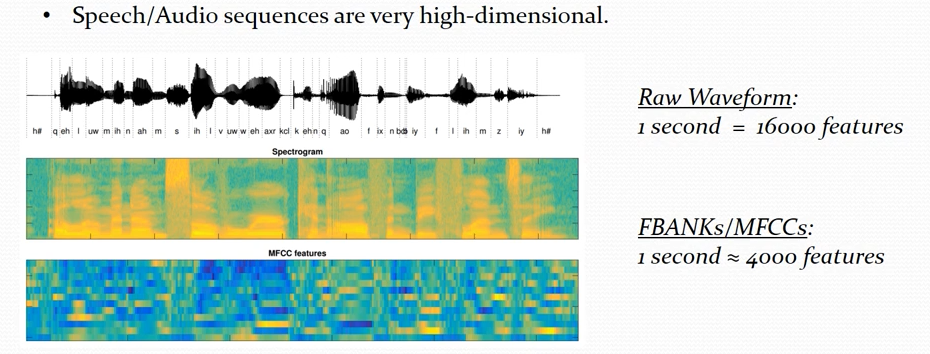
\includegraphics[width=1\linewidth]{images/capture_01.png}
			\caption{A brief introduction to SincNet - Mirco Ravanelli}
			\label{fig:writing-thesis}
		\end{figure}
	\end{itemize}
\end{frame}
\begin{frame}{Vấn đề khi xử lý tín hiệu giọng nói}
	\begin{itemize}
		\item \textbf{Đặc trưng giọng nói có thể bị mất đi} trong quá trình xử lý sóng thô.
		\begin{figure}[H]
			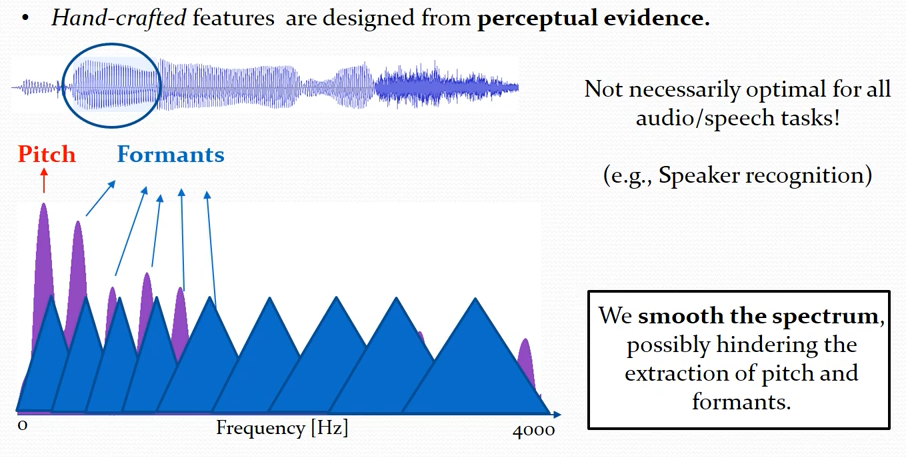
\includegraphics[width=0.9\linewidth]{images/perceptual_evidence.png}
			\caption{A brief introduction to SincNet - Mirco Ravanelli}
			\label{fig:writing-thesis}
		\end{figure}
	\end{itemize}
\end{frame}
\begin{frame}{Vấn đề khi xử lý tín hiệu giọng nói}
	\begin{itemize}
		\item Sự biến mất độ dốc đạo hàm - \textbf{vanishing gradient}
		\begin{figure}[H]
			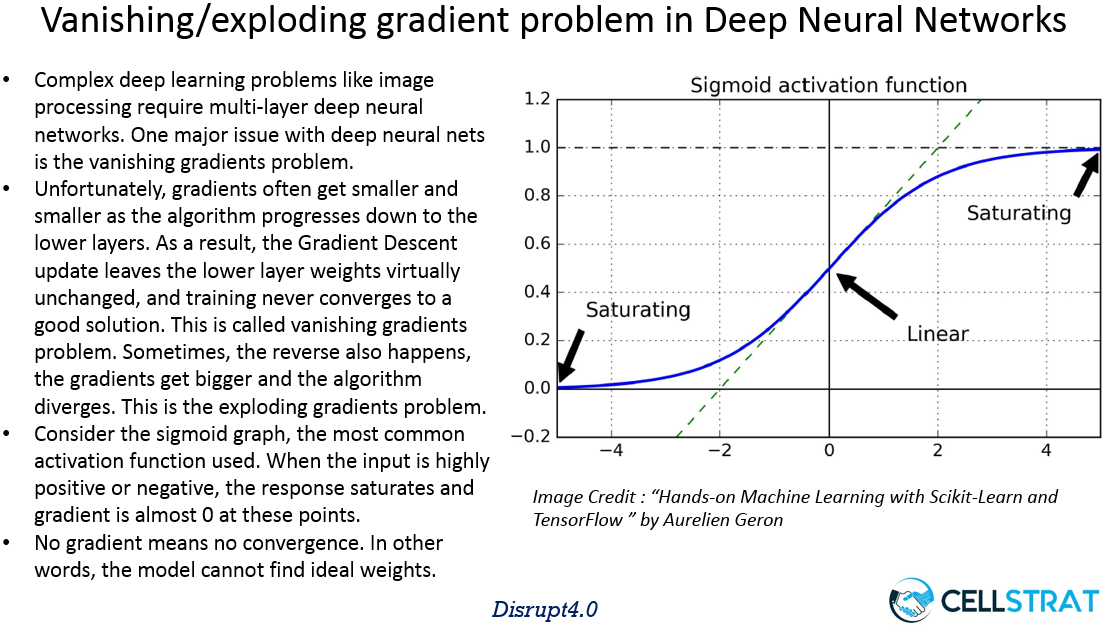
\includegraphics[width=0.75\linewidth]{images/Vanishing-Gradients-in-DNN.png}
			\caption{Vanishing Gradient problem in Deep Neural Networks}
			\label{fig:writing-thesis}
		\end{figure}
	\end{itemize}
\end{frame}
\begin{frame}{Vấn đề khi xử lý tín hiệu giọng nói}
	\begin{itemize}
		\item Các bộ lọc CNNs thường có những \textbf{hình dạng đa băng tần không hợp lý}, khó hiểu.
		\begin{figure}[H]
			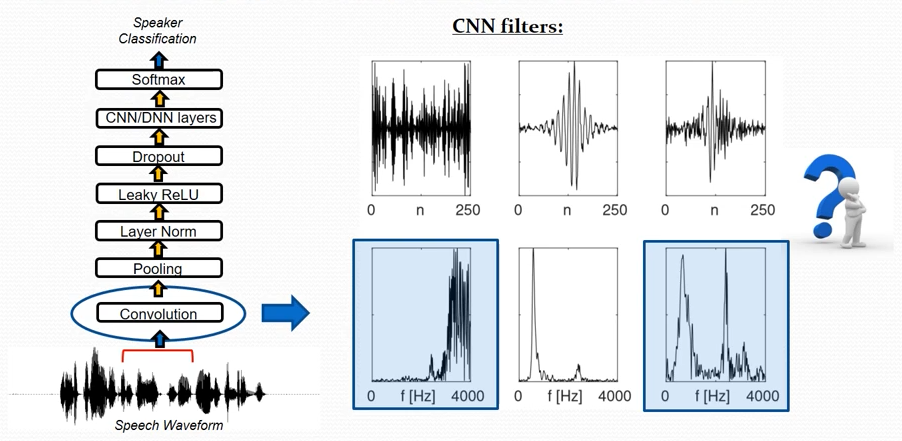
\includegraphics[width=0.9\linewidth]{images/interpretability_problems.png}
			\caption{A brief introduction to SincNet - Mirco Ravanelli}
			\label{fig:writing-thesis}
		\end{figure}
	\end{itemize}
\end{frame}

\section{Kiến trúc mạng SincNet}
\begin{frame}{SincNet}
	\begin{block}{~\vspace{0.7cm}}
		\begin{center}
			\vspace{-0.8cm}
			\begin{tabular}{p{0.45\textwidth}|p{0.45\textwidth}}
				\textcolor{white}{\bf Standard CNN} & \textcolor{white}{\bf SincNet} \\\\
				 $y[n] = x[n] * h[n]$ & $y[n] = x[n] * g[n, \theta]$\\
			\end{tabular}
		\end{center}
	\end{block}
	\textbf{Vấn đề đặt ra: Làm thế nào để chọn được hàm $g(.)$?}
\end{frame}
\begin{frame}{SincNet}
	Ý tưởng để xây dựng hàm $g(.)$: dựa trên bộ lọc băng thông (\textbf{band-pass filters}), chỉ có tần số cắt thấp và cao (low-high cutoff frequencies) được học.
	\begin{figure}[H]
		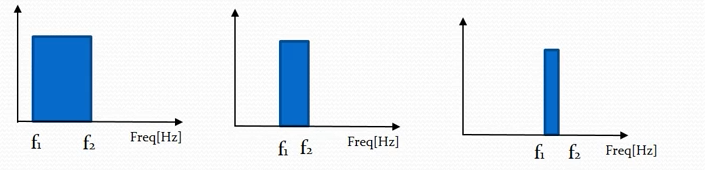
\includegraphics[width=0.9\linewidth]{images/band_passfilters.png}
		\caption{A brief introduction to SincNet - Mirco Ravanelli}
		\label{fig:writing-thesis}
	\end{figure}
\end{frame}
\begin{frame}{SincNet}
	\textbf{Phương pháp thực hiện} Sincnet thực hiện các phép tích chập của nó với hàm $g$, hàm này phụ thuộc vào các tham số $\theta$.
	
	$$y[n] = x[n] * g[n, \theta]$$
	
	Với $f_1$ $f_2$ lần lượt là tần số cắt thấp (low) và cao (high) đã được học, $rect(.)$ là hàm rectangular trong miền tần số.
	
	\begin{gather*}
	G[f, f_1, f_2] = rect\left(\frac{f}{2f_2}\right) -  rect\left(\frac{f}{2f_1}\right)\\ \xrightarrow{\text{Fourier Inverse}}g[n, f_1, f_2] = 2f_2sinc(2\pi f_2 n) - 2f_1sinc(2\pi f_1 n)
	\end{gather*}
\end{frame}
\begin{frame}{SincNet}
	So sánh hình dạng các bộ lọc giữa CNN Filters và SincNet Filters
	\begin{block}{~\vspace{0.7cm}}
		\begin{center}
			\vspace{-0.8cm}
			\begin{tabular}{p{0.45\textwidth}|p{0.45\textwidth}}
				\textcolor{white}{\bf CNN Filters} & \textcolor{white}{\bf SincNet Filters} \\\\
				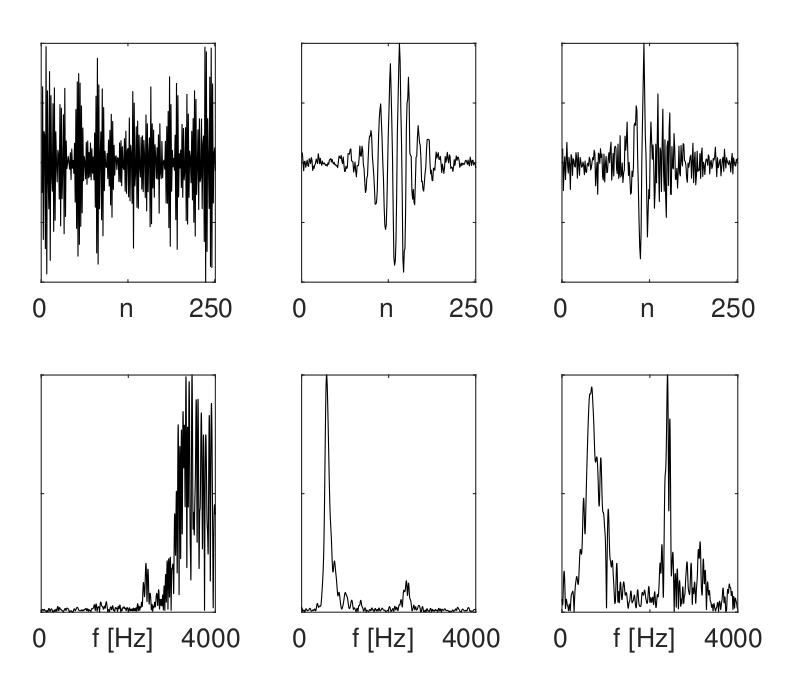
\includegraphics[width=1\linewidth]{images/cnn_filters.png} & 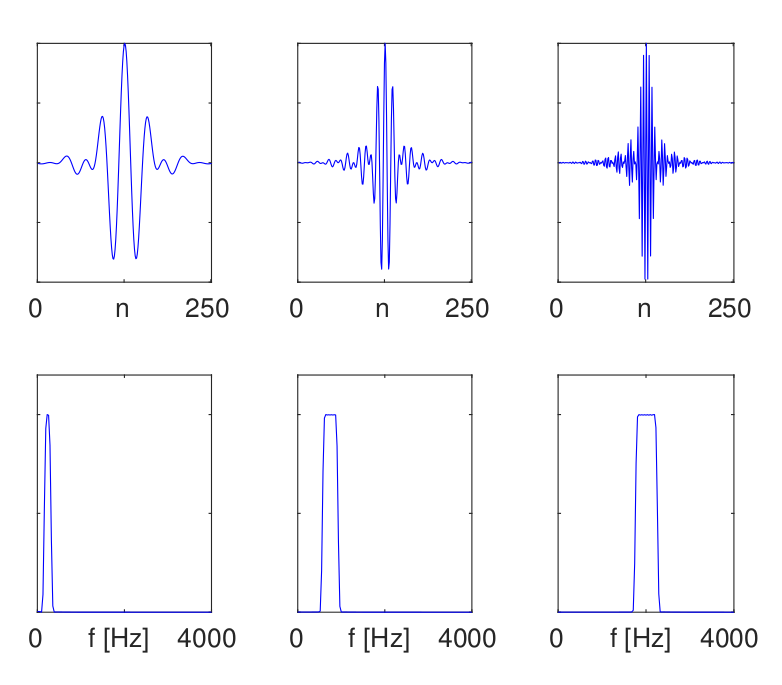
\includegraphics[width=1\linewidth]{images/sincnet_filters.png}\\
			\end{tabular}
		\end{center}
	\end{block}
\end{frame}
\begin{frame}{Kiến trúc mạng SincNet}
	\begin{figure}[H]
		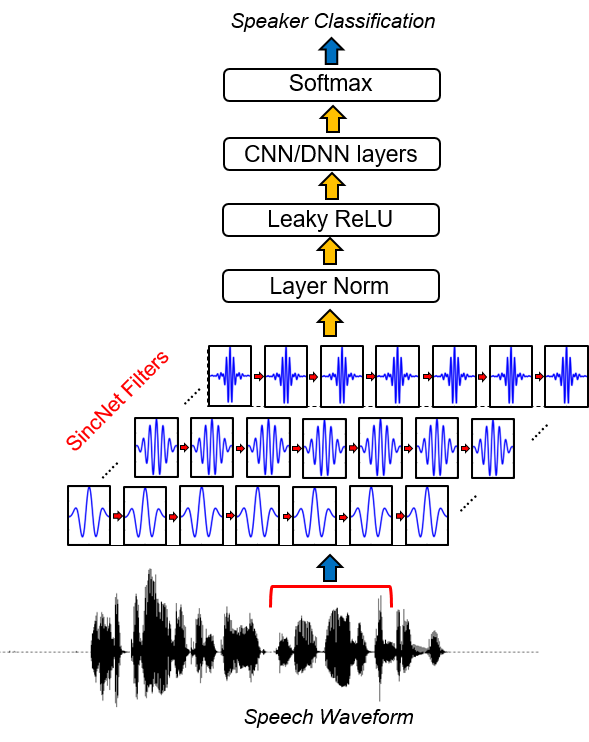
\includegraphics[width=0.4\linewidth]{images/SincNet.png}
		\caption{The SincNet Architecture}
		\label{fig:writing-thesis}
	\end{figure}
\end{frame}
\begin{frame}{Đặc điểm mô hình mạng SincNet}
	\begin{columns}
		\begin{column}{0.47\textwidth}
			\begin{figure}[H]
				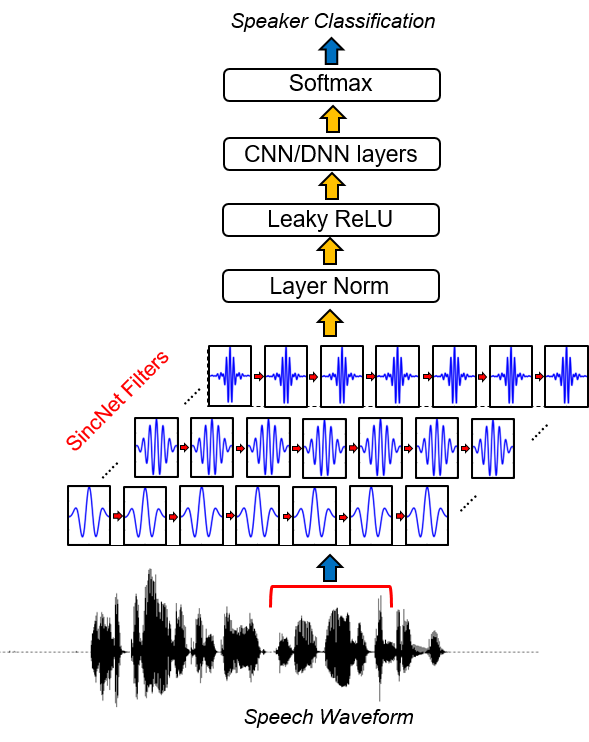
\includegraphics[width=1\linewidth]{images/SincNet.png}
			\end{figure}
		\end{column}
		\begin{column}{0.5\textwidth}
		\begin{itemize}
			\item Tính hội tụ nhanh
			\begin{figure}[H]
				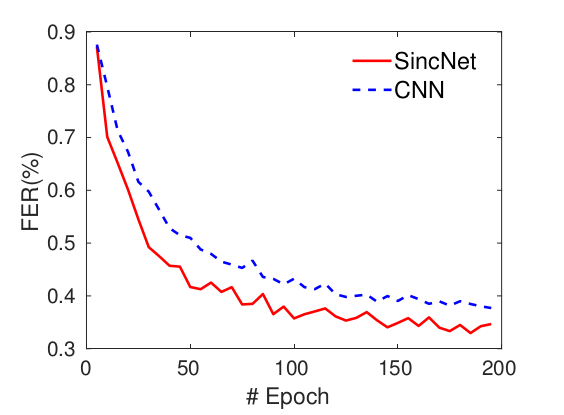
\includegraphics[width=0.9\linewidth]{images/fast_convergence.png}
				\caption{Learning curves}
			\end{figure}
		\end{itemize}
		\end{column}
	\end{columns}
\end{frame}
\begin{frame}{Đặc điểm mô hình mạng SincNet}
	\begin{columns}
		\begin{column}{0.47\textwidth}
			\begin{figure}[H]
				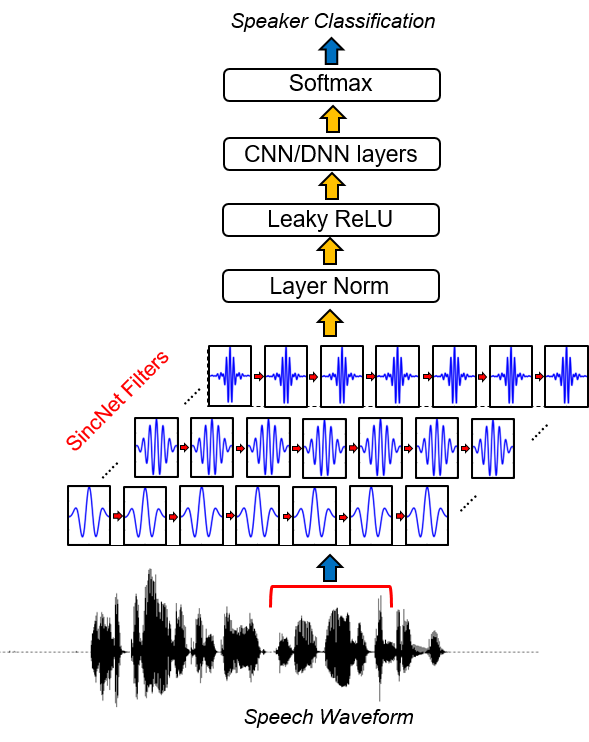
\includegraphics[width=0.9\linewidth]{images/SincNet.png}
			\end{figure}
		\end{column}
		\begin{column}{0.5\textwidth}
			Tính hiệu quả
			\begin{figure}[H]
				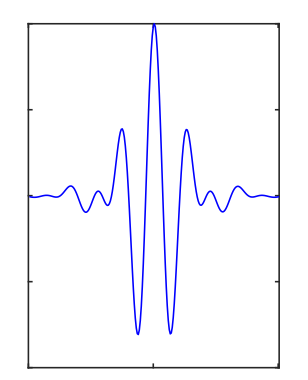
\includegraphics[width=0.75\linewidth]{images/g_symmetric.png}
				\caption{Kernel đối xứng}
			\end{figure}
		\end{column}
	\end{columns}
\end{frame}
\begin{frame}{Đặc điểm mô hình mạng SincNet}
	\begin{columns}
		\begin{column}{0.47\textwidth}
			\begin{figure}[H]
				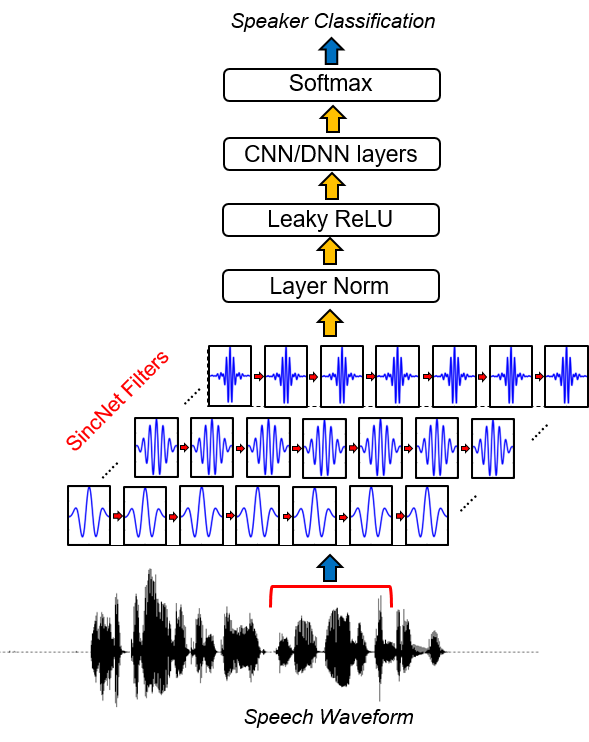
\includegraphics[width=0.9\linewidth]{images/SincNet.png}
			\end{figure}
		\end{column}
		\begin{column}{0.5\textwidth}
			Cần ít tham số cho việc huấn luyện mô hình. \newline
			\begin{itemize}
				\item Với CNN, số tham số là $parameters = F * L$
				\item Với SincNet, số tham số là $parameters = 2F$
			\end{itemize}
		\end{column}
	\end{columns}
\end{frame}
\begin{frame}{Đặc điểm mô hình mạng SincNet}
	\begin{columns}
		\begin{column}{0.47\textwidth}
			\begin{figure}[H]
				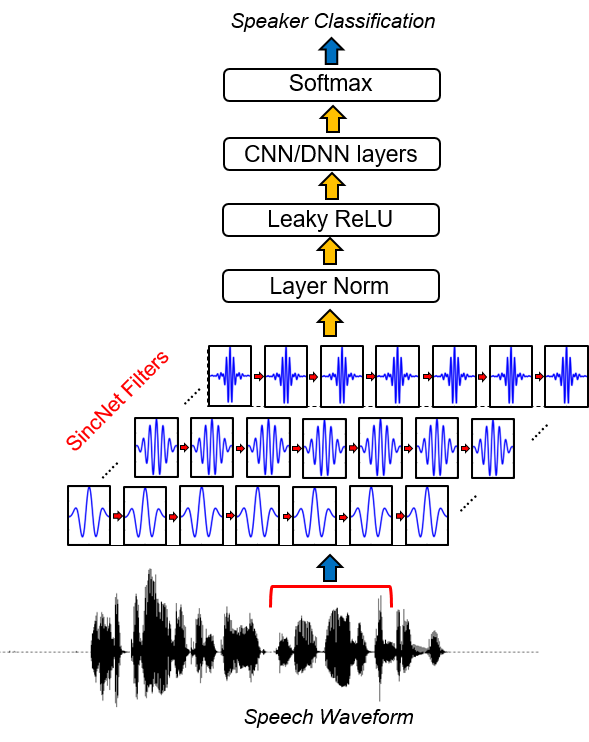
\includegraphics[width=0.9\linewidth]{images/SincNet.png}
			\end{figure}
		\end{column}
		\begin{column}{0.5\textwidth}
			\begin{itemize}
				\item Tính diễn giải
				\begin{figure}[H]
					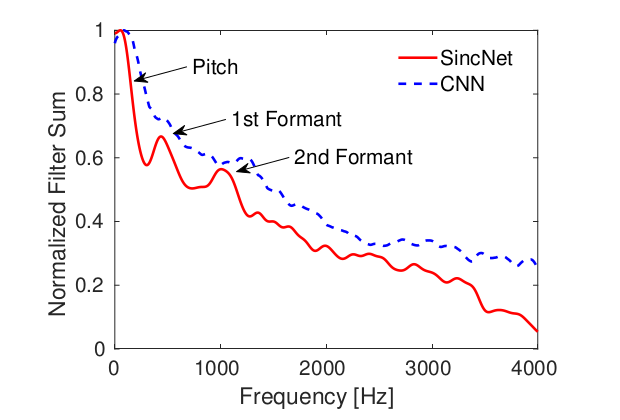
\includegraphics[width=1\linewidth]{images/interpretability.png}
				\end{figure}
			\end{itemize}
		\end{column}
	\end{columns}
\end{frame}

\section{Các kết quả}
\begin{frame}{Các kết quả}
	\begin{columns}
		\begin{column}{0.5\textwidth}
			Các kết quả đối với tác vụ Speaker Identification
			\begin{figure}[H]
				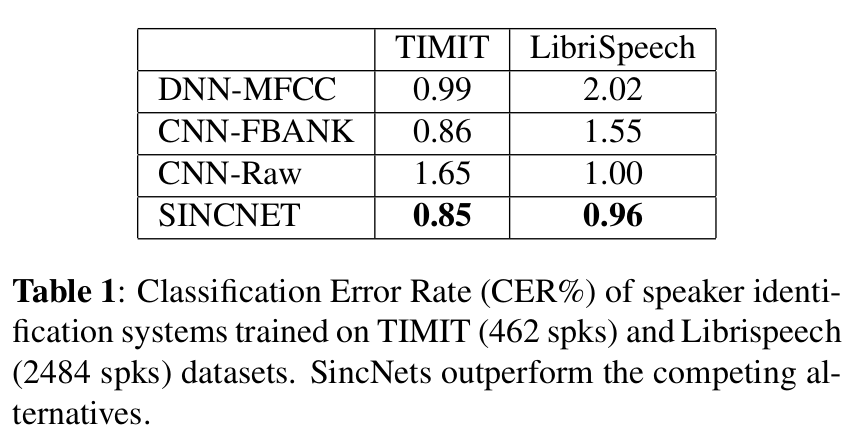
\includegraphics[width=1\linewidth]{images/performance_speaker_identification.png}
			\end{figure}
		\end{column}
		\begin{column}{0.5\textwidth}
			Các kết quả đối với tác vụ Speaker Verification
			\begin{figure}[H]
				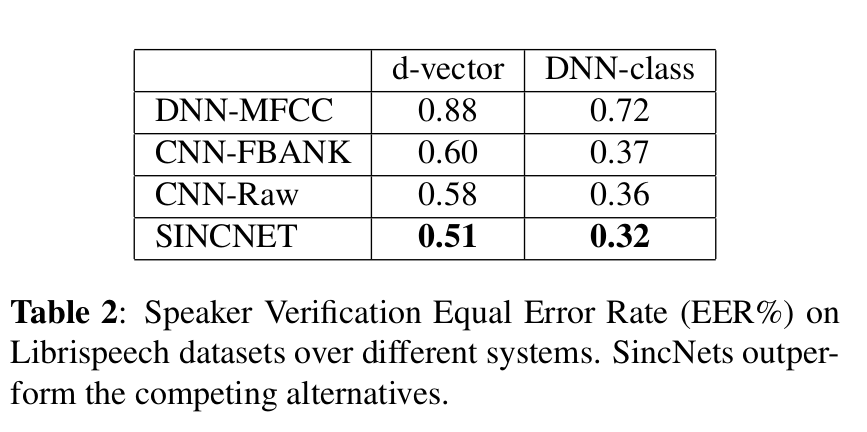
\includegraphics[width=1\linewidth]{images/performance_speaker_verification.png}
			\end{figure}
		\end{column}
	\end{columns}
	\begin{figure}[H]
		\centering
		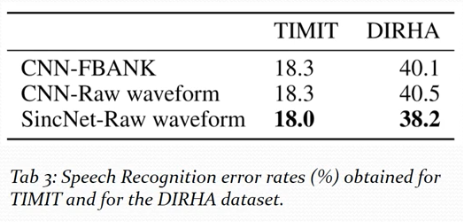
\includegraphics[width=0.65\textwidth]{images/sr_sincnet_result.png}
		\caption{Bảng kết quả Speaker Recognition SincNet trên tập DIRHA}
		\label{fig:writing-thesis}
	\end{figure}	
\end{frame}
\section{Thực nghiệm với SincNet}
\subsection{Chuẩn bị dữ liệu}
\begin{frame}{Chuẩn bị dữ liệu}
	Dữ liệu giọng nói Tiếng Anh
	\begin{itemize}
		\item TIMIT
		\item LibriSpeech
	\end{itemize}
	Dữ liệu giọng nói Tiếng Việt
	\begin{itemize}
		\item Son et al. Dataset + Tự ghi âm bằng micro phone
	\end{itemize}
\end{frame}
\subsection{Phân chia train, test}
\begin{frame}
	Đối với tập TIMIT, Librispeech:  giữ nguyên theo cài đặt của nhóm tác giả
	
	Đối với Son et al. Dataset
	\begin{itemize}
		\item Tập train: mỗi người chọn ra 5 file đầu tiên làm file huấn luyện
		\item Tập test: mỗi người chọn ra 2 file tiếp theo làm file kiểm tra
		\item Tập validation: phần còn lại, dùng để tính toán d-vector
	\end{itemize}
\end{frame}
\subsection{Thông số mô hình}
\begin{frame}
	Các thông số mô hình của nhóm tương tự như thông số được tác giả hướng dẫn từ bài báo
	
	Số lượng epoch dùng cho việc huấn luyện
	\begin{itemize}
		\item TIMIT, Librispeech: 100 epochs
		\item Son Dataset: 300 epochs
	\end{itemize}
\end{frame}
\subsection{Đánh giá mô hình}
\begin{frame}{Đánh giá mô hình}
	Các độ đo đánh giá mô hình
	\begin{itemize}
		\item Tác vụ Speaker Identification
		\begin{itemize}
			\item FER - Frame Error Rate
			\item CER - Classification Error Rate
		\end{itemize}
		\item Tác vụ Speaker Verification
		\begin{itemize}
			\item EER - Equal Error Rate
		\end{itemize}
	\end{itemize}
\end{frame}
\subsection{Kết quả thực nghiệm}
\begin{frame}{Kết quả đánh giá mô hình}
	Các kết quả khi đánh giá mô hình bằng tập TIMIT
	\begin{itemize}
		\item Độ lỗi huấn luyện trung bình mỗi frame $loss\_tr=4.217127$
		\item Giá trị phân lớp sai mức frame $err\_te=0.513561$
		\item Giá trị phân lớp sai mức câu $err\_te\_snt =0.018038$
	\end{itemize}
\end{frame}
\begin{frame}{TIMIT Training Result Visualization}
	\begin{figure}[H]
		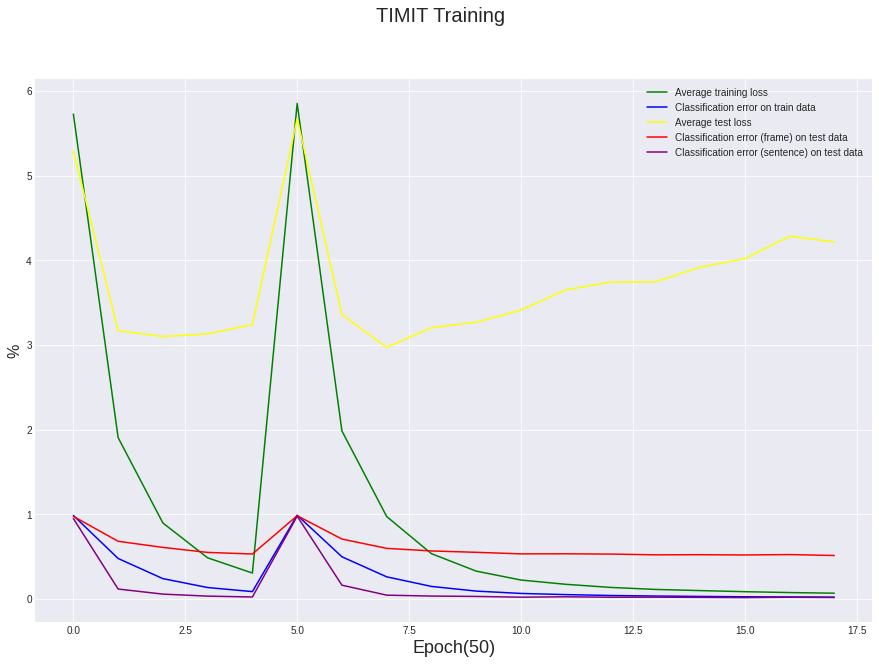
\includegraphics[width=0.8\linewidth]{result/sincnet_timit_plot.png}
		\label{fig:writing-thesis}
	\end{figure}
\end{frame}
\begin{frame}{SincNet on TIMIT Dataset Training Result Visualization}
	\begin{columns}
		\begin{column}{0.47\textwidth}
			\begin{figure}[H]
				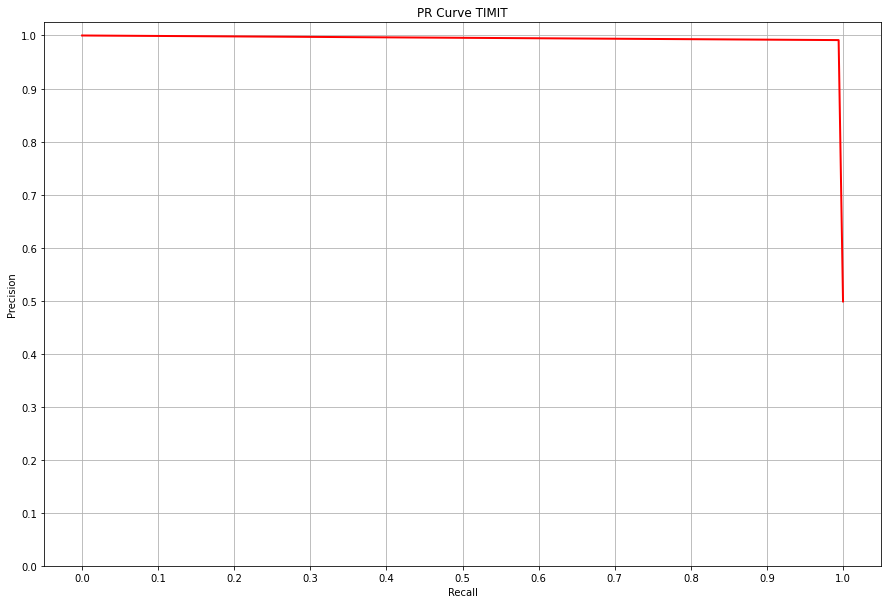
\includegraphics[width=0.9\linewidth]{result/pr_curve_timit.png}
				\caption{Đồ thị PR Curve TIMIT Dataset}
			\end{figure}
			Kết quả đánh giá:
			\begin{itemize}
				\item AP = 0.99
			\end{itemize}
		\end{column}
		\begin{column}{0.5\textwidth}
			\begin{figure}[H]
				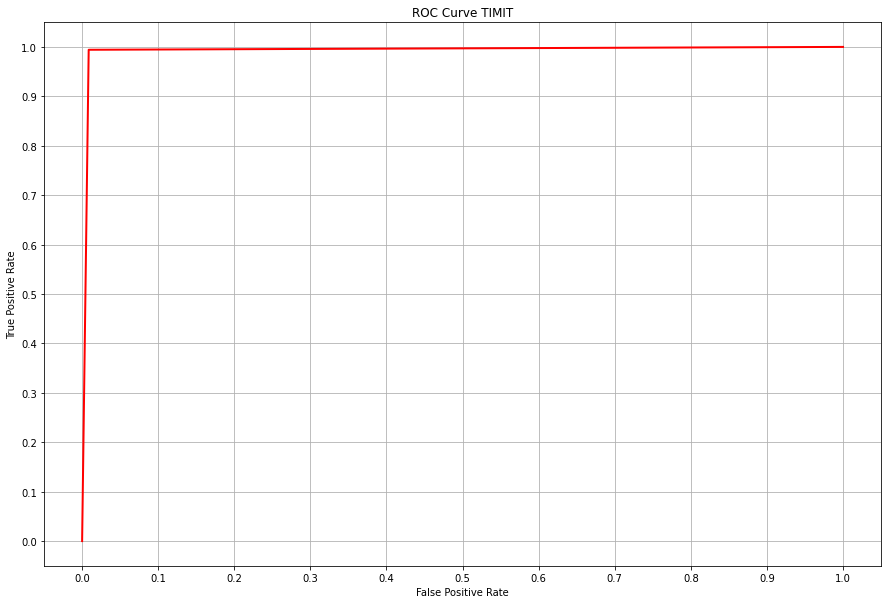
\includegraphics[width=0.9\linewidth]{result/roc_curve_timit.png}
				\caption{Đồ thị ROC Curve TIMIT Dataset}
			\end{figure}
			Kết quả đánh giá:
			\begin{itemize}
				\item EER = 0.0086
				\item AUC = 0.99
			\end{itemize}
		\end{column}
	\end{columns}
\end{frame}
\begin{frame}{Kết quả đánh giá mô hình}
	Các kết quả khi đánh giá mô hình bằng tập Librispeech
	\begin{itemize}
		\item Độ lỗi huấn luyện trung bình mỗi frame $loss\_tr=5.448840$
		\item Giá trị phân lớp sai mức frame $err\_te=0.907977$
		\item Giá trị phân lớp sai mức câu $err\_te\_snt =0.456924$
	\end{itemize}
\end{frame}
\begin{frame}{SincNet on Librispeech Training Result Visualization}
	\begin{figure}[H]
		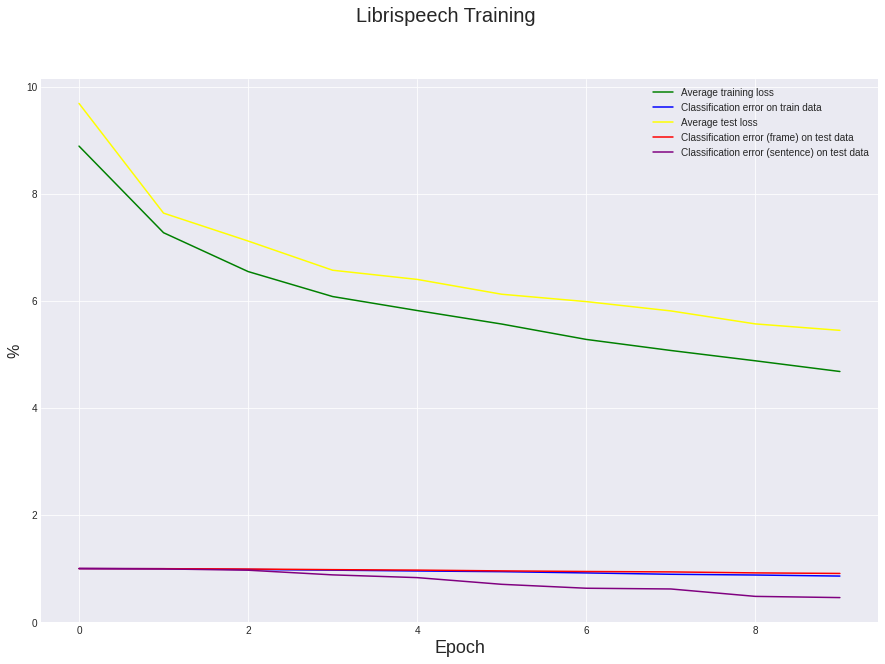
\includegraphics[width=0.8\linewidth]{result/sincnet_librispeech_plot.png}
		\label{fig:writing-thesis}
	\end{figure}
\end{frame}
\begin{frame}{SincNet on Librispeech Dataset Training Result Visualization}
	\begin{columns}
		\begin{column}{0.47\textwidth}
			\begin{figure}[H]
				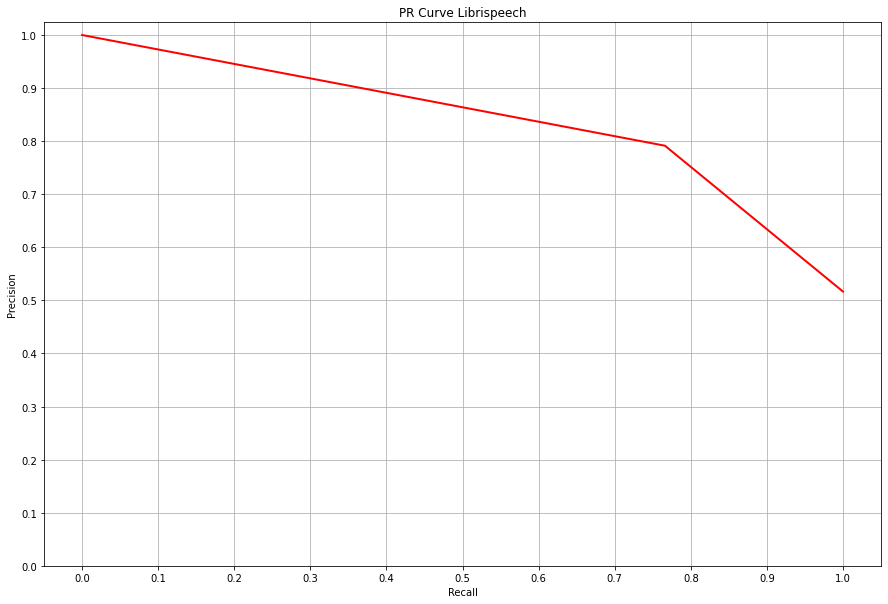
\includegraphics[width=0.9\linewidth]{result/pr_curve_librispeech.png}
				\caption{Đồ thị PR Curve Librispeech Dataset}
			\end{figure}
			Kết quả đánh giá:
			\begin{itemize}
				\item AP = 0.73
			\end{itemize}
		\end{column}
		\begin{column}{0.5\textwidth}
			\begin{figure}[H]
				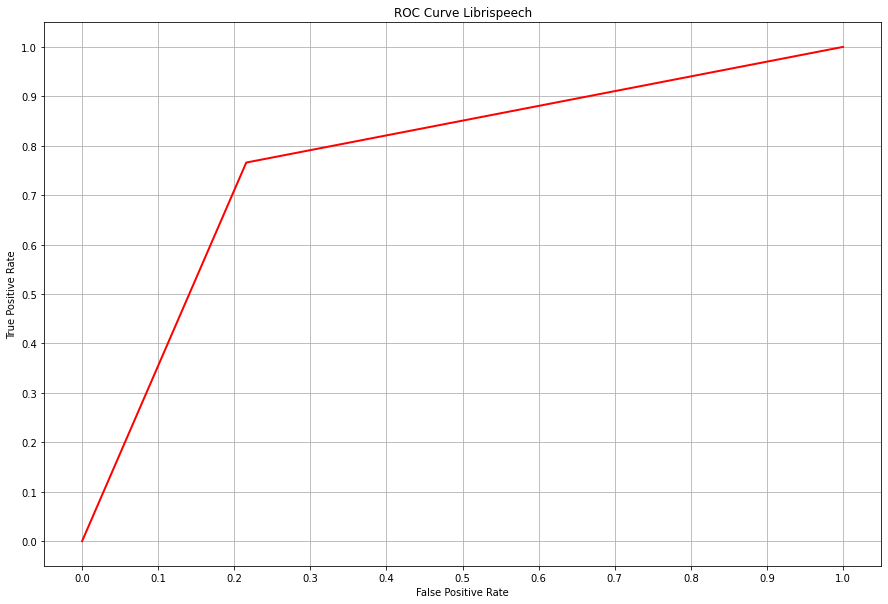
\includegraphics[width=0.9\linewidth]{result/roc_curve_librispeech.png}
				\caption{Đồ thị ROC Curve Librispeech Dataset}
			\end{figure}
			Kết quả đánh giá:
			\begin{itemize}
				\item EER = 0.22
				\item AUC = 0.78
			\end{itemize}
		\end{column}
	\end{columns}
\end{frame}
\begin{frame}{Kết quả đánh giá mô hình}
	Các kết quả khi đánh giá mô hình bằng tập Son et al. Dataset
	\begin{itemize}
		\item Độ lỗi huấn luyện trung bình mỗi frame $loss\_tr=0.113859$
		\item Giá trị phân lớp sai mức frame $err\_te=0.031011$
		\item Giá trị phân lớp sai mức câu $err\_te\_snt =0.000000$
	\end{itemize}
\end{frame}
\begin{frame}{SincNet on Son et al. Dataset Training Result Visualization}
	\begin{figure}[H]
		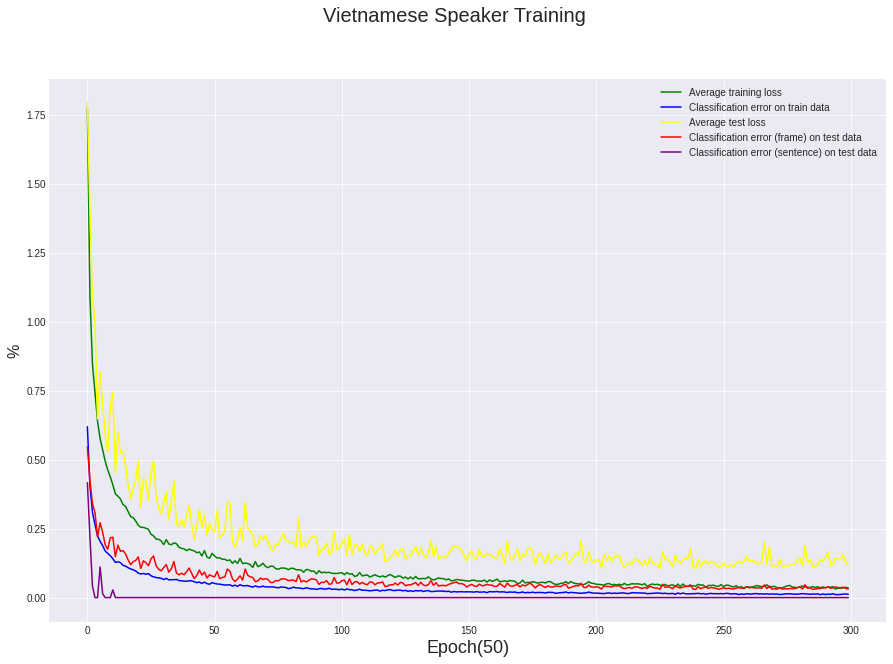
\includegraphics[width=0.8\linewidth]{result/sincnet_vietnamese_plot.png}
		\label{fig:writing-thesis}
	\end{figure}
\end{frame}
\begin{frame}{SincNet on Son et al. Dataset Training Result Visualization}
	\begin{columns}
		\begin{column}{0.47\textwidth}
			\begin{figure}[H]
				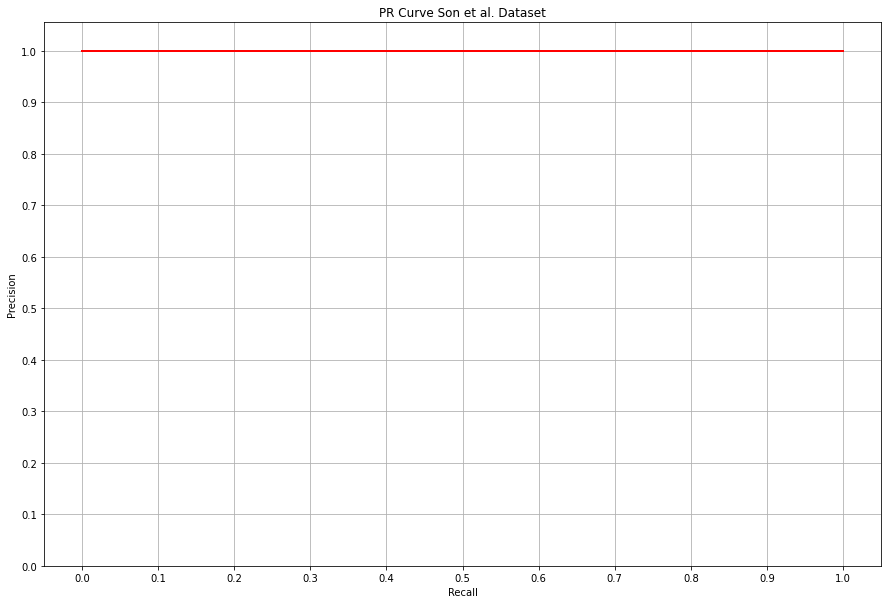
\includegraphics[width=0.9\linewidth]{result/pr_curve_vietnamese.png}
				\caption{Đồ thị PR Curve Son et al. Dataset Dataset}
			\end{figure}
			Kết quả đánh giá:
			\begin{itemize}
				\item AP = 1.0
			\end{itemize}
		\end{column}
		\begin{column}{0.5\textwidth}
			\begin{figure}[H]
				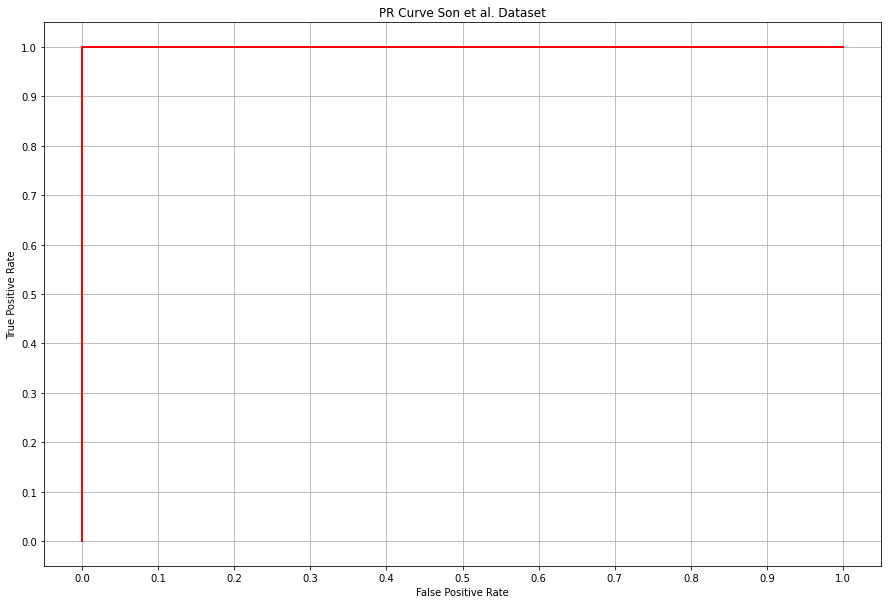
\includegraphics[width=0.9\linewidth]{result/roc_curve_vietnamese.png}
				\caption{Đồ thị ROC Curve Son et al. Dataset Dataset}
			\end{figure}
			Kết quả đánh giá:
			\begin{itemize}
				\item EER = 0.0
				\item AUC = 1.0
			\end{itemize}
		\end{column}
	\end{columns}
\end{frame}
\section{Kết luận}
\begin{frame}{Kết luận}
	Về SincNet Architecture
	\begin{itemize}
		\item Cơ sở lý thuyết Toán học vững vàng.
		\item Tính toán nhanh và gọn nhẹ.
		\item Kết hợp với Deep Learning một cách hiệu quả.
		\item Sử dùng DNN-Class trong đánh giá, cho kết quả đầy hứa hẹn, có độ lỗi EER thấp.
	\end{itemize}
	Nhưng vẫn có hạn chế
	\begin{itemize}
		\item DNN-class tuy có EER thấp nhưng đánh đổi nhiều sự linh hoạt so với d-vectors
	\end{itemize}
\end{frame}

\section{Tài liệu tham khảo}
\begin{frame}{Tài liệu tham khảo}
	\nocite{*}
	\bibliography{references}\newpage\cleardoublepage
	\bibliographystyle{plain}
\end{frame}


\begin{frame}{Q\&A}
	\begin{center}
		\Huge Cảm ơn thầy và các bạn đã theo dõi và lắng nghe
	\end{center}
\end{frame}

\end{document}